\documentclass[11pt]{article} % 
\usepackage[pdftex]{graphicx}
\usepackage{fullpage}
\usepackage{graphicx}
\usepackage{graphics}
\usepackage{psfrag}
\usepackage{pgf}
\usepackage{color}
\usepackage{verbatim}
\usepackage{tikz}
\usetikzlibrary{arrows,automata}
\usepackage[latin1]{inputenc}
\usepackage{amsthm}
\usepackage{amsmath,amssymb}
\usepackage{enumerate}
\setlength{\textwidth}{6.5in}
\setlength{\textheight}{9in}
\newcommand{\cP}{\mathcal{P}}
\newcommand{\N}{\mathbb{N}}
\newcommand{\Z}{\mathbb{Z}}
\newcommand{\R}{\mathbb{R}}
\newcommand{\Q}{\mathbb{Q}}
\newcommand{\C}{\mathbb{C}}
\newcommand{\tab}{\;\;\;\;\;}
\newcommand{\inv}{^{-1}}

\begin{document}

\hfill Robert Johns

\hfill October 16, 2013

\begin{center} {\Large CSCI 426: Simulation}\\{\large Homework 4}\end{center}

\begin{enumerate}

%1
\item[4.1.2] Prove Theorem 4.1.1 for the $1/(n-1)$ form of the sample variance.  That is, prove that if the root-mean-square value associated with any value of $x$ is $$d(x) = \sqrt{\frac{1}{n-1}\sum_{i=1}^n(x_i-x)^2}$$ then the smallest possible root-mean square value of $d(x)$ is $d(\bar{x}) = s$, and this value is achieved if and only if $x = \bar{x}$.

{\bf Proof:} First, let us prove the second part. We can see that, since $d(x)$ is a well-defined and injective function, from the definition of the variance and standard deviation (at least the $1/(n-1)$ version we're working with), we have that $d(\bar{x}) = \sqrt{s^2} = s$, and $d\inv(s) = \bar{x}$.  

Minimality is trickier.  We're trying to prove that $s = d(\bar{x})$ is the minimum possible value of our function.  Any value on the real number line will be either $\bar{x}$ or some constant away from $\bar{x}$.  Without loss of generality, we can call this constant $k$ and examine the cases $d(\bar{x} + k)$ and $d(\bar{x} - k)$, showing that both obtain values larger than $s$.  If we can do that, we're done.

Let us examine $d(\bar{x} - k)$ first.  We have
 $$d(\bar{x} - k) = \sqrt{\frac{1}{n-1}\sum_{i-1}^n(x_i - (\bar{x} - k))^2} = \sqrt{\frac{1}{n-1}\sum_{i-1}^n(x_i - \bar{x} + k)^2}$$ 
$$= \sqrt{\frac{1}{n-1}\sum_{i-1}^n(x_i^2 - 2x^i\bar{x} + \bar{x}^2 + 2kx_i -2k\bar{x} + k^2)}$$ 
$$= \sqrt{\frac{1}{n-1}\sum_{i-1}^n(x_i - \bar{x})^2 + \frac{2k}{n-1}\sum_{i=1}^n(x_i -\bar{x}) + \frac{nk^2}{n-1}}$$ 
$$ = \sqrt{s^2 + \frac{2k}{n-1}(n\bar{x} - n\bar{x}) + \frac{nk^2}{n-1}} = \sqrt{s^2 + \frac{nk^2}{n-1}}$$ which will be greater than $s$ as $n$ and $k$ are both positive constants.  

Now let us examine $d(\bar{x} + k)$.  We have 
$$d(\bar{x} - k) = \sqrt{\frac{1}{n-1}\sum_{i-1}^n(x_i - (\bar{x} + k))^2} = \sqrt{\frac{1}{n-1}\sum_{i-1}^n(x_i - \bar{x} - k)^2}$$ 
$$= \sqrt{\frac{1}{n-1}\sum_{i-1}^n(x_i^2 - 2x^i\bar{x} + \bar{x}^2 - 2kx_i  + 2k\bar{x} + k^2)}$$ 
$$= \sqrt{\frac{1}{n-1}\sum_{i-1}^n(x_i - \bar{x})^2 + \frac{2k}{n-1}\sum_{i=1}^n(\bar{x} - x_i) + \frac{nk^2}{n-1}}$$ 
$$ = \sqrt{s^2 + \frac{2k}{n-1}(n\bar{x} - n\bar{x}) + \frac{nk^2}{n-1}} = \sqrt{s^2 + \frac{nk^2}{n-1}}$$ which will be greater than $s$ as $n$ and $k$ are both positive constants.  So we now know that $d(\bar{x})$ is the minimum value of $d(x)$, and that $d(\bar{x}) = s$, proving the theorem. 

%2
\item[4.2.9] Generate a random-variate demand sample size $n = 10000$ as $$d_i = \texttt{Equilikely(5,25) + Equilikely(5,25);}$$  for $i = 1, 2, \dots, n$.

\begin{enumerate}

\item Why is the sample mean about 30?

{\bf Solution:} Since the two random variates are independent (the values do not depend on each other), we can take their means and sum them to obtain the mean of $d_i$.  From the handy chart in the front of the book, we have that the mean of an $Equilikely(a,b)$ model is $\frac{a+b}{2}$, which in this case is $\frac{5+25}{2} = 15$.  So we have that the mean of $d_i$ is $15 + 15 = 30$.  Therefore, as long as it's implemented properly, the mean of any appropriately-sized sample of the sum of two $Equilikely(5,25)$ variates should be around 30.

\item Why is the sample standard deviation about $\sqrt{220/3}$?

{\bf Solution:} In the same way as {\bf(a)} above, we can sum the two variates' variances, as they are independent of one another, and then take the square root to get the standard deviation.  We have (again from the handy chart in the front of the book) that the formula for the variance of an $Equilikely(a,b)$ model is $\sigma^2 = \frac{(b-a+1)^2 - 1}{12}$, which in this case is $\frac{(25 - 5 + 1)^2-1}{12} = \frac{21^2-1}{12} = \frac{440}{12} = \frac{110}{3}$.  So then the mean of $d_i$ will be $\frac{110}{3} + \frac{110}{3} = \frac{220}{3}$, and thus the standard deviation is $\sqrt{\frac{220}{3}}$.  Therefore, as long as it's implemented properly, the standard deviation of any appropriately-sized sample of the sum of any two $Equilikely(2,25)$ variates should be around $\sqrt{\frac{220}{3}}$.

\item Why is the shape of the histogram approximately triangular?

{\bf Solution:} Our histogram is approximately triangular, with the peak around the mean (which is around 30).  Intuitively, this makes sense for the same reason that the distribution of the sum of the rolls of two fair dice is triangular, with the apex around the mean at 7; because no matter what you roll first, the second roll can always be a value which, when added to your first roll, gives you 7, but your options become more and more limited as you move outwards to 2 and 12.  Similarly, in this example, you can always get 30 no matter what your first $Equilikely(5,25)$ random variate is, but 30 cannot be obtained when either variate is 5, and so on until the only way you can get 10 is with two 5s, and the only way you can get 50 is with two 25s.
\end{enumerate}

\newpage

%3
\item[4.3.4] Generate a random-variate sample $x_1, x_2, \ldots x_n$ of size $n = 10000$ as follows:

\texttt{for (}$i$\texttt{ = 1; }$i$\texttt{ <= }$n$\texttt{; }$i$\texttt{++)}

$\tab x_i$ \texttt{ = Random() + Random();}

\begin{enumerate}

\item Use program \texttt{cdh.c} to construct a 20-bin continuous-data histogram.

{\bf Solution:} When the modified code (given at end of assignment) is run, we get the following histogram:

$\begin{array}{|l|l|l|l|l|}\hline
\textrm{bin} & \textrm{midpoint} & \textrm{count} & \textrm{proportion} & \textrm{density} \\\hline
    1 &       0.050 &        56 &       0.006 &       0.056\\
    2 &       0.150 &       140 &       0.014 &       0.140\\
    3 &       0.250 &       265 &       0.026 &       0.265\\
    4 &       0.350 &       352 &       0.035 &       0.352\\
    5 &       0.450 &       403 &       0.040 &       0.403\\
    6 &       0.550 &       540 &       0.054 &       0.540\\
    7 &       0.650 &       658 &       0.066 &       0.658\\
    8 &       0.750 &       733 &       0.073 &       0.733\\
    9 &       0.850 &       901 &       0.090 &       0.901\\
   10 &       0.950 &      1009 &       0.101 &       1.009\\
   11 &       1.050 &       970 &       0.097 &       0.970\\
   12 &       1.150 &       804 &       0.080 &       0.804\\
   13 &       1.250 &       717 &       0.072 &       0.717\\
   14 &       1.350 &       625 &       0.062 &       0.625\\
   15 &       1.450 &       548 &       0.055 &       0.548\\
   16 &       1.550 &       467 &       0.047 &       0.467\\
   17 &       1.650 &       369 &       0.037 &       0.369\\
   18 &       1.750 &       230 &       0.023 &       0.230\\
   19 &       1.850 &       168 &       0.017 &       0.168\\
   20 &       1.950 &        45 &       0.004 &       0.045\\\hline
   \end{array}$

Additionally, this histogram has the following properties:

sample size $= 10000$,
mean $= 1.000$,
standard deviation $= 0.409$

\item Can you find an equation that seems to fit the histogram density well?

{\bf Solution:} We seem to have a triangular distribution, defined piecewise by 
$$f(x) = \left\{\begin{array}{cc}
x/10 & 0 \le x < 1 \\
.2 - x/10  & 1 \le x < 2\\
0 & \textrm{otherwise}
\end{array}\right.$$
which gives us the following figure:

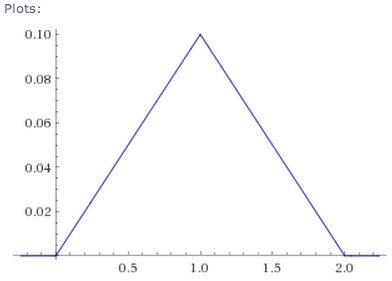
\includegraphics[scale = .5]{one}

\end{enumerate}

\end{enumerate}

\end{document}